% Options for packages loaded elsewhere
\PassOptionsToPackage{unicode}{hyperref}
\PassOptionsToPackage{hyphens}{url}
%
\documentclass[
]{article}
\usepackage{amsmath,amssymb}
\usepackage{geometry} 
\usepackage{iftex}
\ifPDFTeX
  \usepackage[T1]{fontenc}
  \usepackage[utf8]{inputenc}
  \usepackage{textcomp} % provide euro and other symbols
\else % if luatex or xetex
  \usepackage{unicode-math} % this also loads fontspec
  \defaultfontfeatures{Scale=MatchLowercase}
  \defaultfontfeatures[\rmfamily]{Ligatures=TeX,Scale=1}
\fi
\usepackage{lmodern}
\ifPDFTeX\else
  % xetex/luatex font selection
\fi
% Use upquote if available, for straight quotes in verbatim environments
\IfFileExists{upquote.sty}{\usepackage{upquote}}{}
\IfFileExists{microtype.sty}{% use microtype if available
  \usepackage[]{microtype}
  \UseMicrotypeSet[protrusion]{basicmath} % disable protrusion for tt fonts
}{}
\makeatletter
\@ifundefined{KOMAClassName}{% if non-KOMA class
  \IfFileExists{parskip.sty}{%
    \usepackage{parskip}
  }{% else
    \setlength{\parindent}{0pt}
    \setlength{\parskip}{6pt plus 2pt minus 1pt}}
}{% if KOMA class
  \KOMAoptions{parskip=half}}
\makeatother
\usepackage{xcolor}
\usepackage{graphicx}
\makeatletter
\def\maxwidth{\ifdim\Gin@nat@width>\linewidth\linewidth\else\Gin@nat@width\fi}
\def\maxheight{\ifdim\Gin@nat@height>\textheight\textheight\else\Gin@nat@height\fi}
\makeatother

\setkeys{Gin}{width=\maxwidth,height=\maxheight,keepaspectratio}
% Set default figure placement to htbp
\makeatletter
\def\fps@figure{htbp}
\makeatother
\setlength{\emergencystretch}{3em} % prevent overfull lines
\providecommand{\tightlist}{%
  \setlength{\itemsep}{0pt}\setlength{\parskip}{0pt}}
\setcounter{secnumdepth}{-\maxdimen} % remove section numbering
\ifLuaTeX
  \usepackage{selnolig}  % disable illegal ligatures
\fi
\usepackage{bookmark}
\IfFileExists{xurl.sty}{\usepackage{xurl}}{} % add URL line breaks if available
\urlstyle{same}
\hypersetup{
  hidelinks,
  pdfcreator={LaTeX via pandoc}}

\title{\phantomsection\label{_m3fsboosfdtx}{}

\phantomsection\label{_gbgxfwdo0k7x}{}Práctica 2. Ejercicio Grupal

\phantomsection\label{_xror403oixh4}{}Aplicación para Gestión de
Empresa}
\author{}
\date{}

\begin{document}
\maketitle

\textbf{Integrantes del grupo}

\begin{itemize}
\item
  Carmen Chunyin Fernández Núñez
\item
  Pablo García Guijosa
\item
  Marta Xiaoyang Moraga Hernández
\item
  Jesús Navarrete Caparrós
\end{itemize}
 \pagebreak
\section{Índice}\label{uxedndice}

\hyperref[uxedndice]{\textbf{Índice 2}}

\hyperref[descripciuxf3n]{\textbf{Descripción 3}}

\hyperref[diagrama]{\textbf{Diagrama 4}}

\hyperref[modelo]{\textbf{Modelo 5}}

\begin{quote}
\hyperref[departamento]{Departamento}

\hyperref[elementoempresa]{ElementoEmpresa}

\hyperref[empleado]{Empleado}

\hyperref[empleadobuilder]{EmpleadoBuilder}

\hyperref[empleadomediotiempobuilder]{EmpleadoMedioTiempoBuilder}

\hyperref[empleadotiempocompletobuilder]{EmpleadoTiempoCompletoBuilder}

\hyperref[tipobuider]{TipoBuider}
\end{quote}

\hyperref[controlador]{\textbf{Controlador 15}}

\begin{quote}
\hyperref[director]{Director}
\end{quote}

\hyperref[vista]{\textbf{Vista 18}}

\begin{quote}
\hyperref[empleadowidget]{EmpleadoWidget}

\hyperref[listaelementoswidget]{ListaElementosWidget}

\hyperref[main]{main}
\end{quote}

\hyperref[funcionamiento]{\textbf{Funcionamiento 31}}

\hyperref[conclusiuxf3n]{\textbf{Conclusión 35}}
\pagebreak
\section{Descripción}\label{descripciuxf3n}

En esta práctica hemos revisado y mejorado el ejercicio planteado
anteriormente. Nuestro objetivo es simular la organización de una
empresa, utilizando el patrón Builder para construir diferentes tipos de
empleados y el Composite para manejar la jerarquía de la empresa. Hemos
realizado modificaciones principalmente en el Patrón Composite, ya que
el enfoque utilizado en la práctica anterior no era completamente
correcto.

Ahora, en lugar de tener múltiples arrays en la clase Departamento para
almacenar diferentes tipos de elementos de la empresa, utilizamos un
único array que guarda objetos del tipo Elemento Empresa. Además, hemos
incluido en la clase Director un array de Elemento Empresa para que sea
el Director quien maneje todo lo relacionado con la empresa.

El objetivo de esta práctica, además de mejorar el código anterior, es
crear una interfaz para nuestro proyecto utilizando Flutter y Dart. En
esta interfaz se mostrará la jerarquía de la empresa, la cual será
controlada únicamente por el director. Además, se podrán añadir y
eliminar los empleados y departamentos desde la interfaz.

\section{Diagrama}\label{diagrama}

{[}Imagen UML en la siguiente página{]}
\newgeometry{left=1in,bottom=0.1in,top=0.2in}
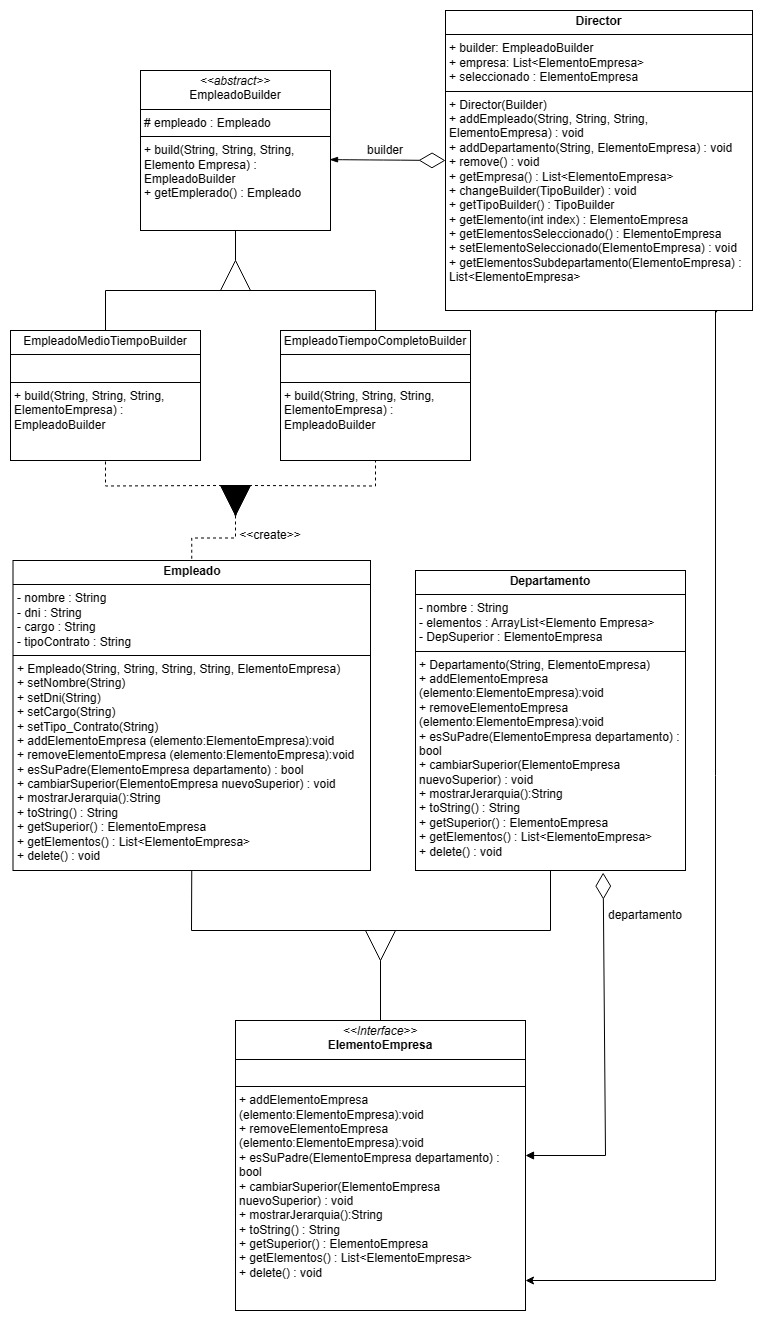
\includegraphics[width=5.90522in,height=10.22222in]{imagenes/UML.jpg}
\restoregeometry
\section{Modelo}\label{modelo}

A la hora de modificar el código, hemos tenido ciertos problemas pues el
cambio de java a flutter, además de mejorar el código, ha implicado
tener que cambiar bastantes cosas. En muchas variables y métodos hemos
tenido que poner ? ya que flutter no deja que una variable sea nula a
menos que pongamos la interrogación. También hemos tenido que añadir una
clase TipoBuilder, que es un enumerador, para utilizar un menú
desplegable en la interfaz y seleccionar el tipo de Builder que deberá
utilizar el director.

\subsubsection{Departamento}\label{departamento}

La clase Departamento hereda de la clase ElementoEmpresa y tiene un
array para almacenar diferentes tipos de ElementoEmpresa. También tiene
un ElementoEmpresa DepSuperior que indica cual es el Departamento
Superior al que pertenece, si lo hubiese.

En Dart, cuando se quiere llamar al método de un objeto que podría ser
nulo se debe llamar con una interrogación. Por ello, al adaptarlo de
Java, aunque se compruebe antes que es nulo y gestionemos que hacer en
tal caso, muchos de los métodos deben ser llamados de la forma
departamento?.metodo(). En tal caso de que el Departamento sea nulo, el
método no se ejecuta.

Esto es una cosa que afecta bastante cuando es necesario usar el
Departamento Superior (DepSuperior). Ya que podría ser nulo (el
ElementoEmpresa no pertenece a un departamento) o no.

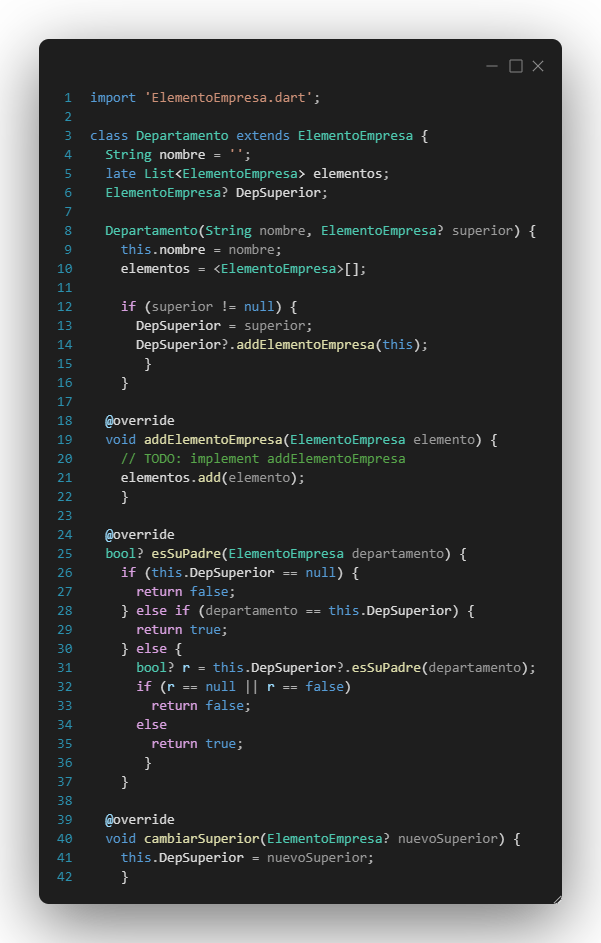
\includegraphics[width=5.90522in,height=9.26389in]{imagenes/Departamento1.png}

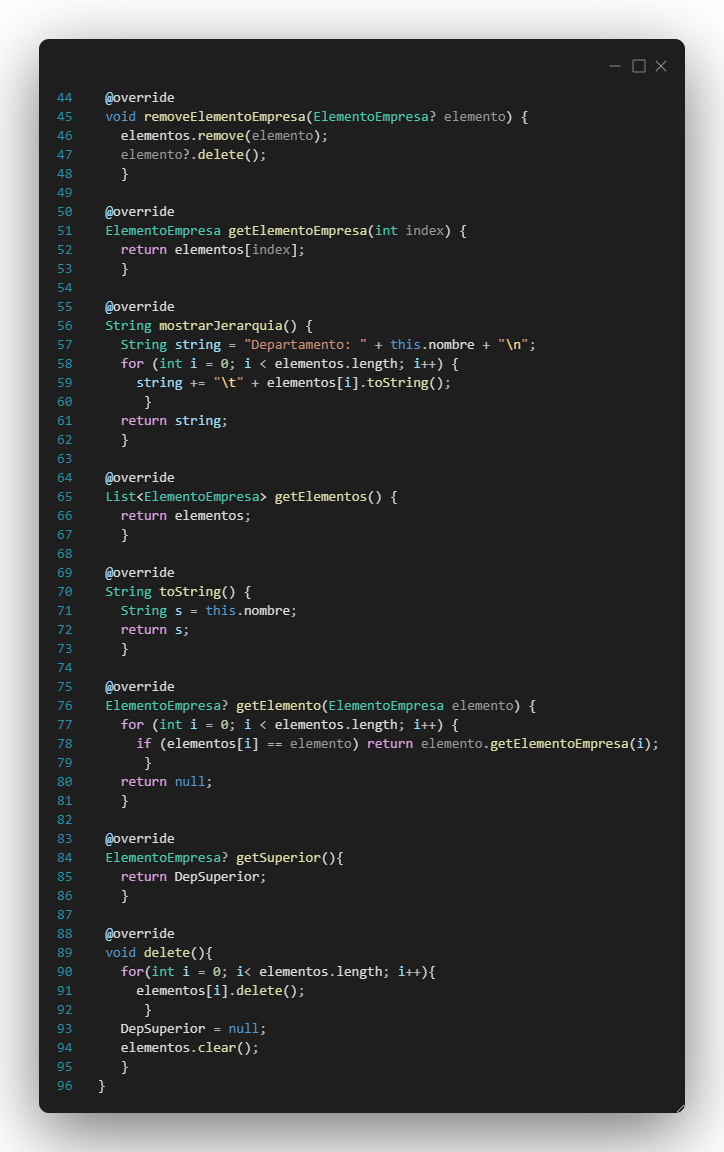
\includegraphics[width=5.90522in,height=9.40278in]{imagenes/Departamento2.png}

\subsubsection{ElementoEmpresa}\label{elementoempresa}

Esta interfaz, definida como clase abstracta en dart (puesto que los
interface de Dart obligan a incluir implementación \{\}, aunque esta
esté vacía, y por tanto esta es una adaptación más fiel a la intención
del código original de Java), es la que implementan el Departamento y
Empleado. En ella, se definen los métodos a utilizar por los objetos
tipo ElementoEmpresa. Gracias a que existe ElementoEmpresa, hay cohesión
entre Empleado y Departamento, y Departamento puede gestionar tener
ambos en su interior. Esta es la razón de que se eligiera utilizar el
patrón Composite para el problema diseñado.

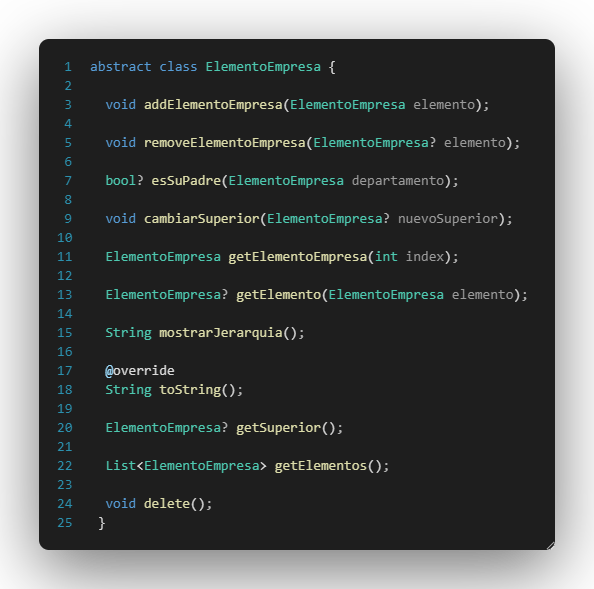
\includegraphics[]{imagenes/ElementoEmpresa.png}

\subsubsection{Empleado}\label{empleado}

La clase Empleado hereda de la clase ElementoEmpresa, además para crear
este tipo de objetos, se utilizan los Builders. Estos Builders los
utilizará el direcctior según sea necesario. La mayoría de los métodos
de ElementoEmpresa, están implementdos como errores, pues hay muchas
funcionalidades que los Empleados no deberían poder hacer.

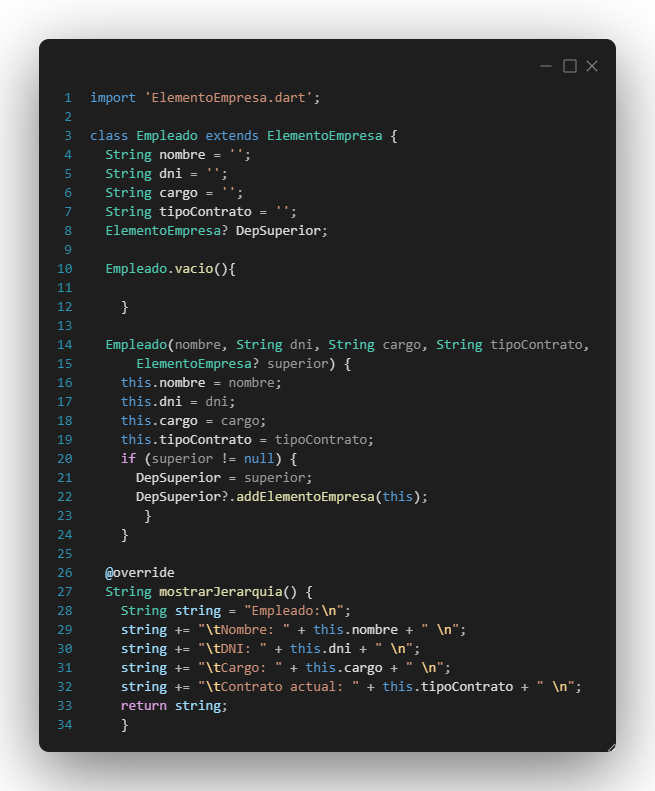
\includegraphics[width=5.90522in,height=7.125in]{imagenes/Empleado1.png}
\pagebreak
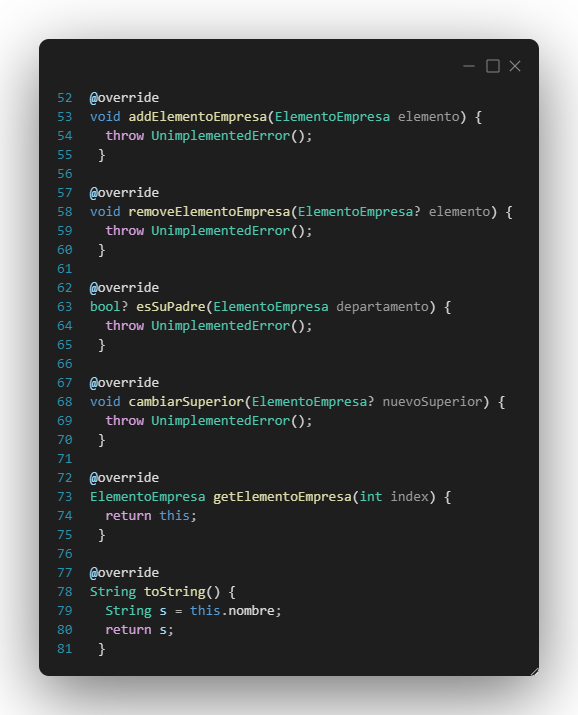
\includegraphics[width=5.90522in,height=7.30556in]{imagenes/Empleado2.png}
\pagebreak
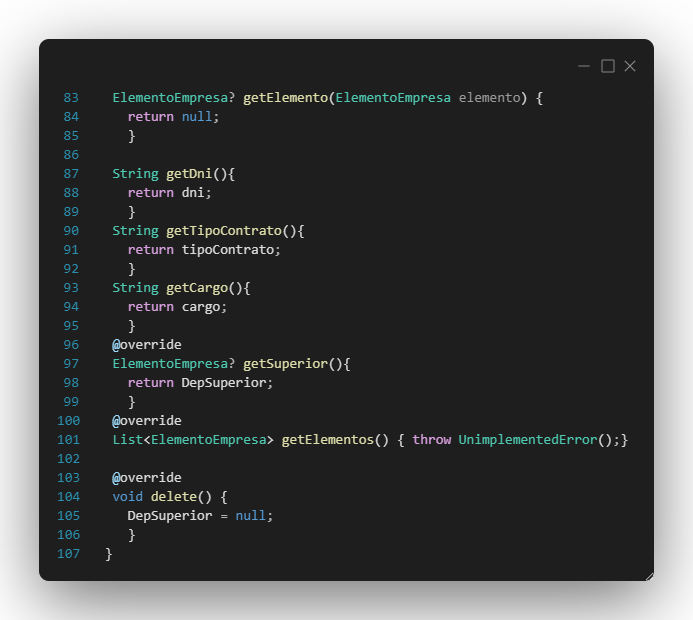
\includegraphics[width=5.90522in,height=5.27778in]{imagenes/Empleado3.png}

\subsubsection{EmpleadoBuilder}\label{empleadobuilder}

Este clase abstracta es la que permite construir el objeto Empleado, en
el director se elige que tipo de Builder se quiere utilizar y se llama a
la función build del Builder especificado

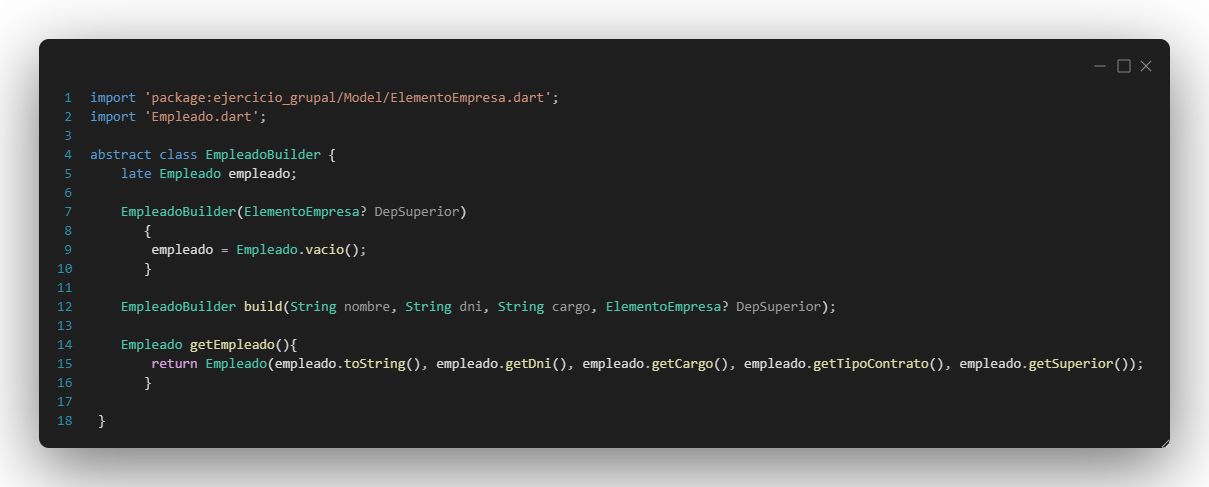
\includegraphics[width=5.90522in,height=2.375in]{imagenes/EmpleadoBuilder.png}

\subsubsection{EmpleadoMedioTiempoBuilder}\label{empleadomediotiempobuilder}

Hereda de EmpleadoBuilder y crea Empleados con un contrato de Medio
Tiempo

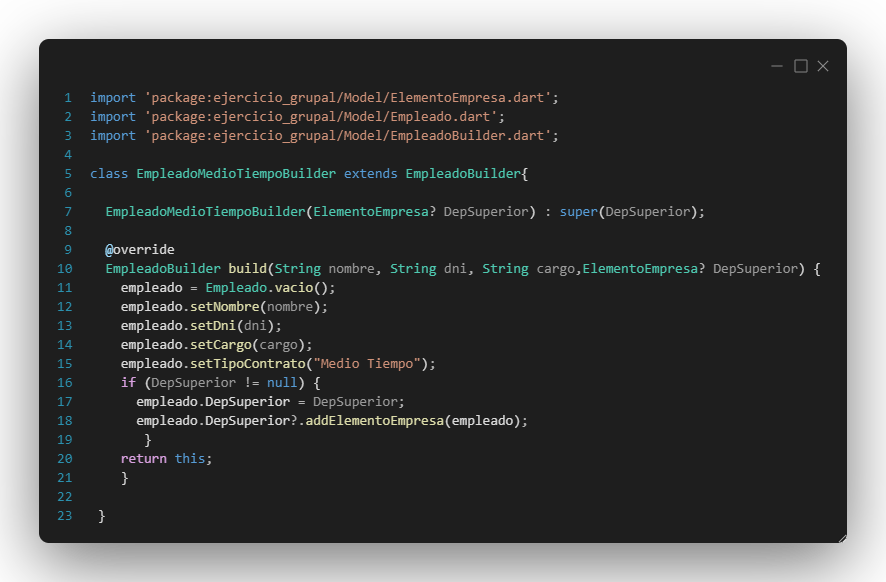
\includegraphics[width=5.90522in,height=3.875in]{imagenes/MedioTiempo.png}

\subsubsection{EmpleadoTiempoCompletoBuilder}\label{empleadotiempocompletobuilder}

Hereda de EmpleadoBuilder y crea Empleados con un contrato de Tiempo
Completo

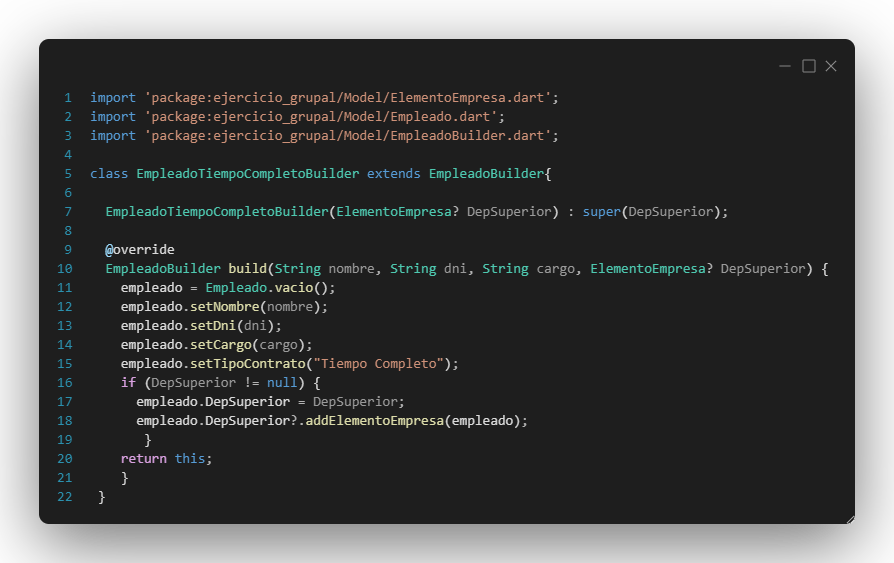
\includegraphics[width=5.90522in,height=3.72222in]{imagenes/TiempoCompleto.png}

\subsubsection{TipoBuider}\label{tipobuider}

Esta clase está creada para facilitar en la interfaz la selección del
builder a utilizar.

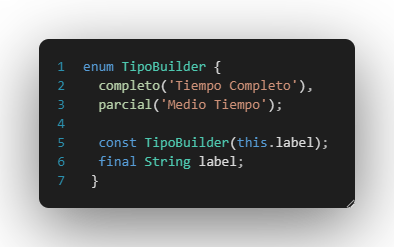
\includegraphics[width=4.10417in,height=2.57292in]{imagenes/TipoBuilder.png}

\section{Controlador}\label{controlador}

\subsubsection{Director}\label{director}

El director es el que se encarga de controlar toda la empresa. Esta
clase tiene un objeto builder, para construir los empleados, un array de
ElementoEmpresa para manejar la jerarquía de la empresa y un objeto
ElementoEmpresa que sería el objeto sobre el cual se está trabajando
actualmente. El objeto seleccionado lo hemos creado porque al ser el
atributo empresa un array, era más difícil trabajar sobre él, y para
poder guardar sobre qué objeto se desea trabajar.

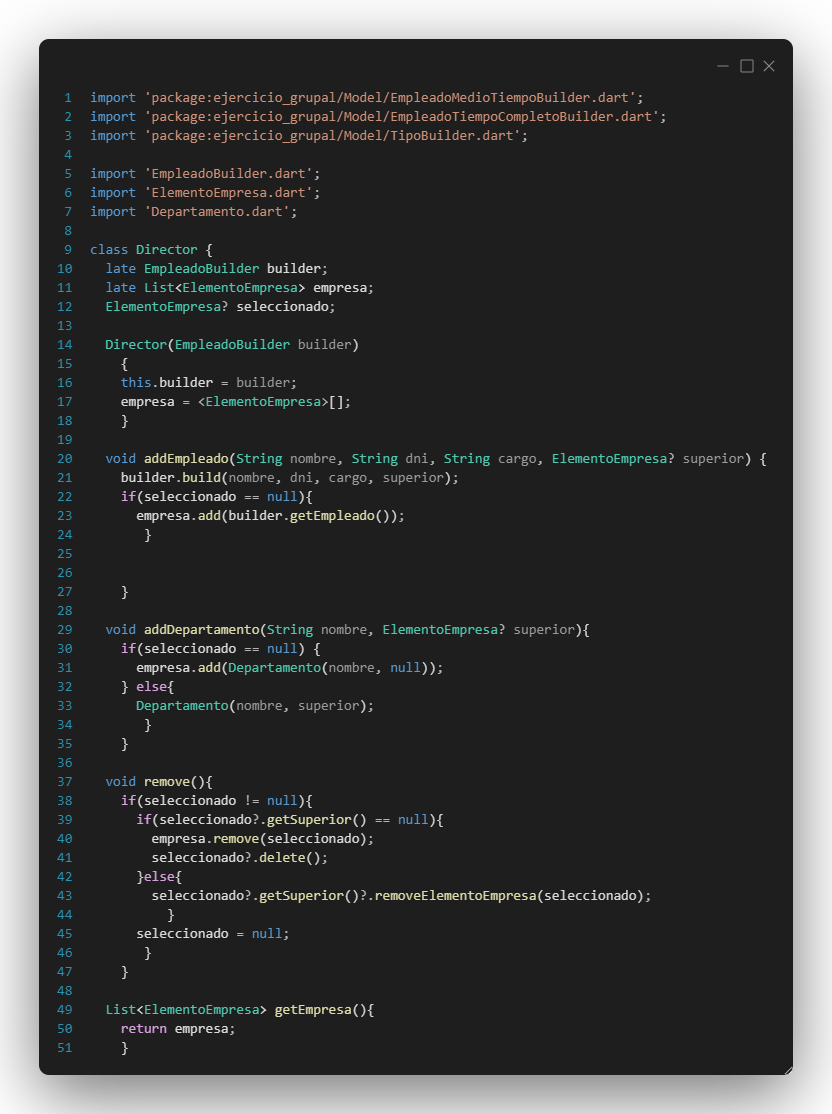
\includegraphics[width=5.90522in,height=7.90278in]{imagenes/Director1.png}
\pagebreak
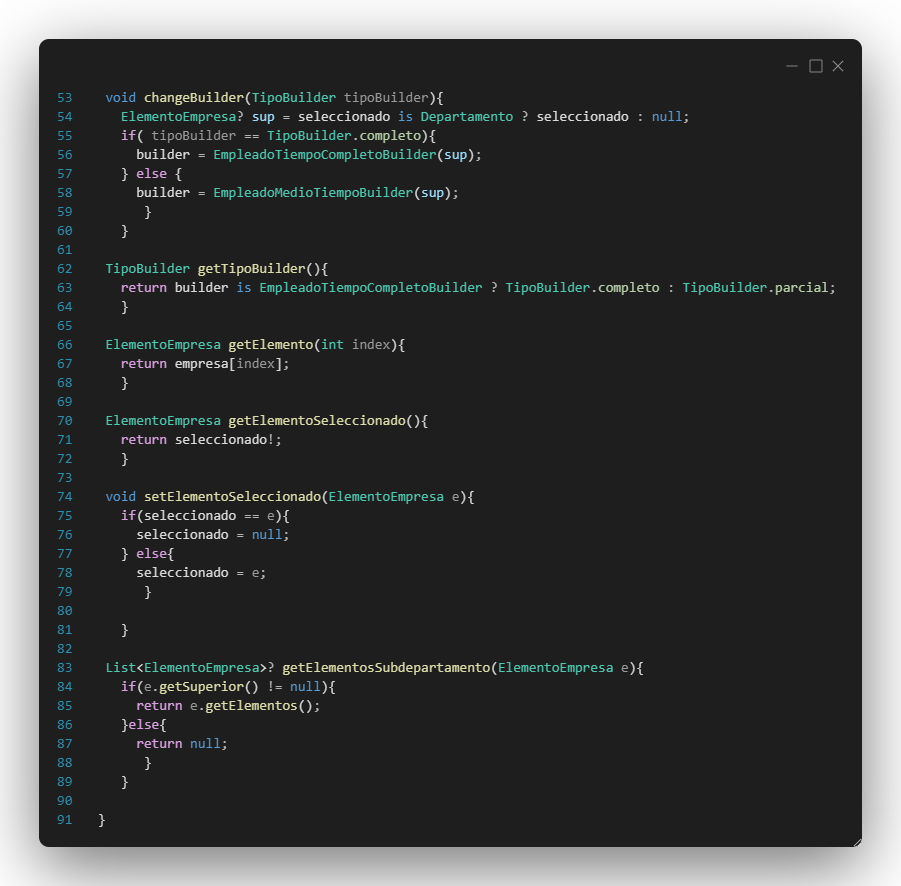
\includegraphics[width=5.90522in,height=5.80556in]{imagenes/Director2.png}

\section{Vista}\label{vista}

\subsubsection{\texorpdfstring{\protect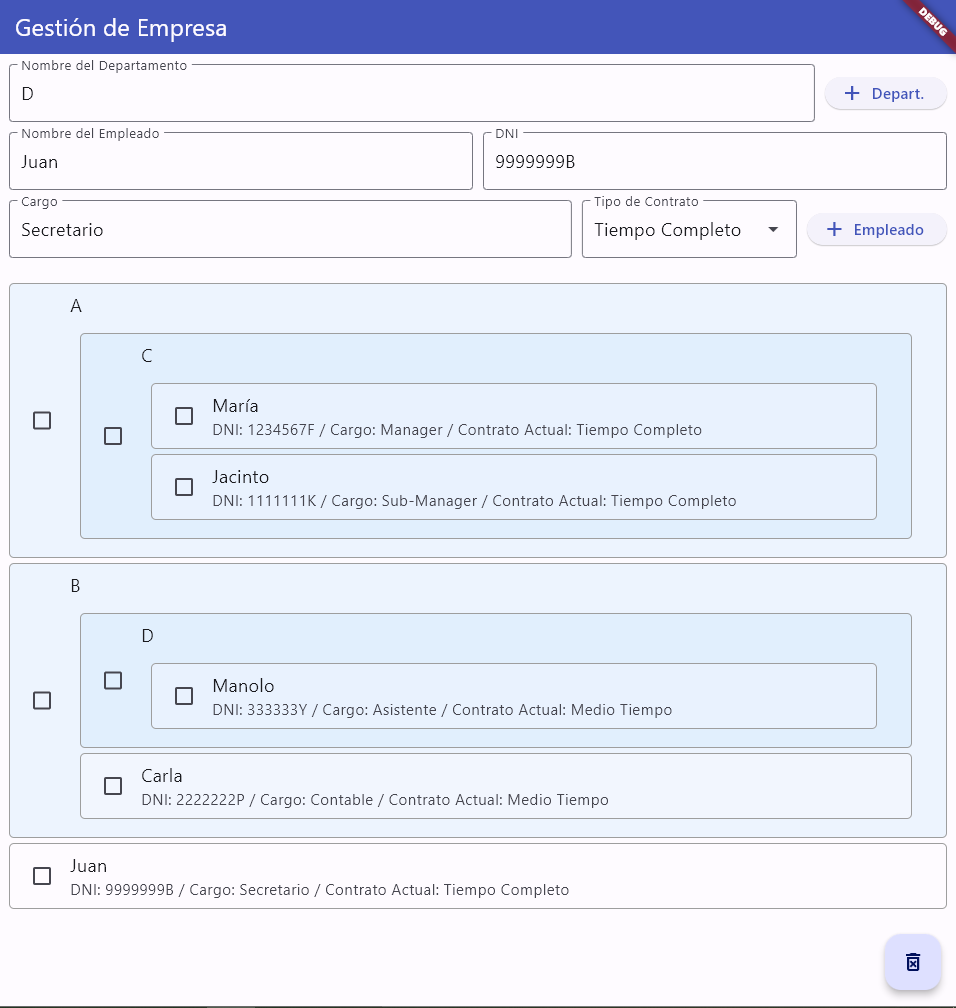
\includegraphics[width=5.90625in,height=6.17408in]{imagenes/Vista.png}}{}}\label{section}

Para la vista, como se indica en la práctica, se utilizan los Widgets de
Flutter.

\subsubsection{EmpleadoWidget}\label{empleadowidget}

Este es un StatelessWidget que crea un Text del empleado dado. Lo
utiliza el Widget que está encargado de generar la lista de
ElementoEmpresa para añadirlo cuando hace falta. Necesita que sea pasado
un empleado, puesto que los departamentos carecen de todos esos datos,
pero una alternativa sería que se pasará un ElementoEmpresa en el que se
utilizará casting para crear una variable local Empleado que utilizamos.
Esta alternativa es mejor puesto que así sólo acepta el objeto que puede
utilizar, permitiendo detectar errores, y deberá ser quién lo use quién
se encargue de pasar el objeto correcto.

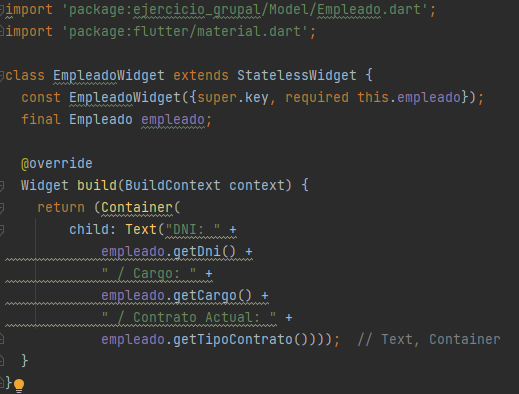
\includegraphics[width=5.40625in,height=4.10417in]{imagenes/EmpleadoWidget.png}

\subsubsection{ListaElementosWidget}\label{listaelementoswidget}

Es un Widget que se encarga de mostrar una lista de ElementoEmpresa.
Requiere de dicha lista, para mostrar los elementos, y de un Director,
que actúa como controlador. Algunas explicaciones:

\begin{itemize}
\item
  ListView.builder es lo que permite generar de forma automática,
  definiendo un objeto que se usa de base, los elementos de la lista de
  longitud variable. El valor de itemCount es cuántos elementos
  generará, por lo que se establece a la longitud de la lista. El
  itemBuilder utiliza un index para identificar qué elemento de la lista
  se está creando.
\item
  Padding, como su nombre indica nos permite darle a su hijo espacio de
  relleno, y así espaciar los elementos al gusto.
\item
  ListTile representa un elemento de la ListView. Su color de fondo
  variará dependiendo de si puede tener hijos o no. Esta consulta se la
  hacemos al director.
\item
  Checkbox permite al usuario seleccionar un elemento y a la vez mostrar
  una retroalimentación de ello. Su valor se obtiene consultando al
  director.estaSeleccionado(ElementoEmpresa). Cuando se pulsa la
  CheckBox, se llama director.setElementoSeleccionado(ElementoEmpresa) y
  este método es el encargado de que director recuerde el seleccionado
  (o lo olvide si la casilla ya estaba marcada y se quiere
  deseleccionar). Después de eso, utiliza un callback y esto notifica al
  padre del cambio. Utilizar el callback es necesario, porque si no, un
  elemento marcado con anterioridad no se actualizará y seguirá
  apareciendo como el seleccionado al usuario aunque internamente no lo
  sea.
\item
  El subtítulo será otro ListaElementosWidgets si el elemento puede
  tener hijos (pasamos el mismo director y la lista de ElementoEmpresa
  que tiene el elemtento) o será EmpleadoWidget, en caso contrario.
\item
  La lista de ElementoEmpresa de un Departamento se comporta igual que
  la lista original.
\item
  El callback que se pasa por el constructor de ListaElementosWidget es
  necesario por la creación reiterada de ListaElementosWidget, permite
  avisar al padre hasta llegar a la raíz de la primera invocación, y
  pedir que se actualice el estado de este. Como se explicó
  anteriormente, sin esto no se mostraría la información de forma
  correcta al usuario.
\end{itemize}

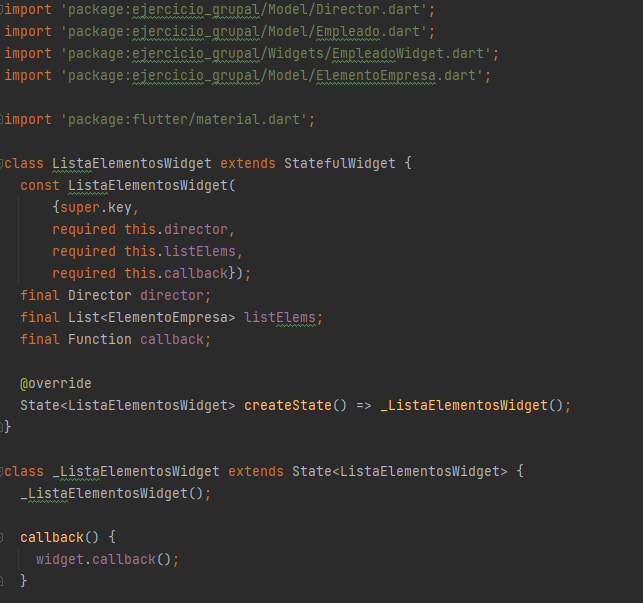
\includegraphics[width=5.90522in,height=5.54167in]{imagenes/ListaElementosWidget1.png}

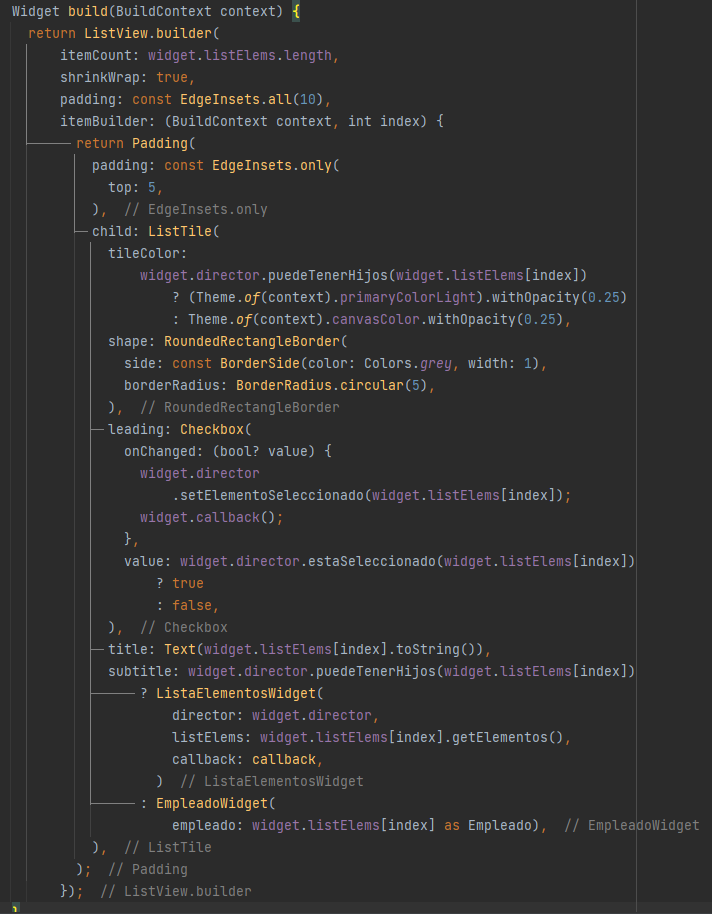
\includegraphics[width=5.90522in,height=7.58333in]{imagenes/ListaElementosWidget2.png}

\subsubsection{main}\label{main}

El main llama a ListaElementosWidget y define el callback original que
actualiza el estado con setState. Los hijos del main simplemente llaman
al callback del padre hasta llegar aquí. Las funciones que se hacen por
pulsar los botones son básicamente pedirle al director que añada un
elemento, obteniendo los datos de los controladores, o que elimine un
elemento. El director es el que internamente intentará eliminar el que
tenga guardado como seleccionado o comprobará si debe añadir el
ElementoEmpresa a su lista o a la de algún elemento de esta. Sobre los
Widgets:

\begin{itemize}
\item
  Flexible permite que los TextField adapten su tamaño dependiendo de
  los elementos con los que compartan Row o Column.
\item
  Extended es necesario (junto a shrinkWrap: true, en el ListView) para
  poder mostrar una ListView en el interior de una columna. Esto es
  porque el comportamiento predeterminado de ListView no se adapta
  correctamente a Row o Column, ya que es Scrollable.
\item
  Para espaciar columnas y filas hay varias formas, como envolver cada
  elemento con Padding. En este caso utilizamos un SizezBox cuando sea
  necesario, ya que es más simple encontrar las separaciones a simple
  vista.
\end{itemize}

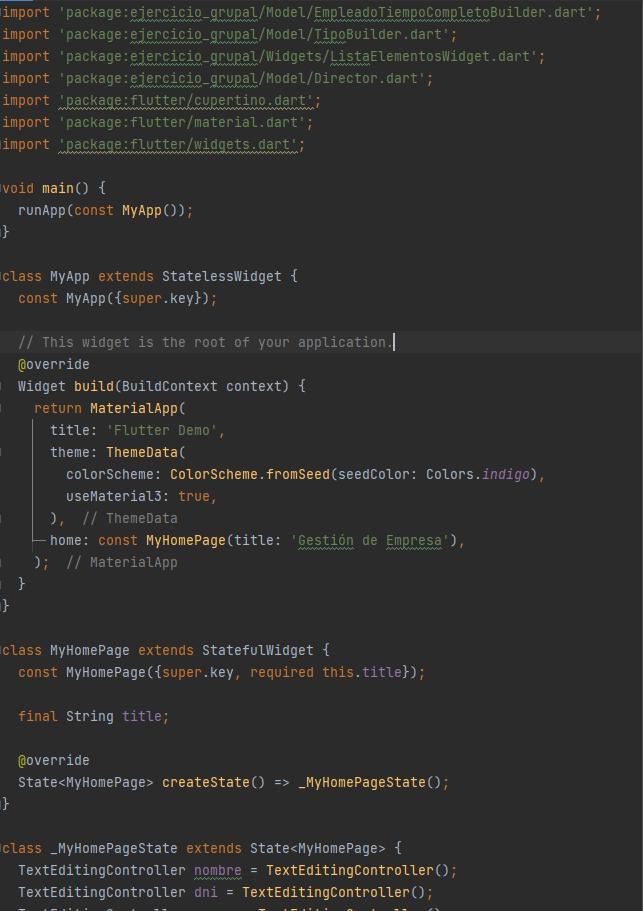
\includegraphics[width=5.90625in,height=7.65139in]{imagenes/main1.png}

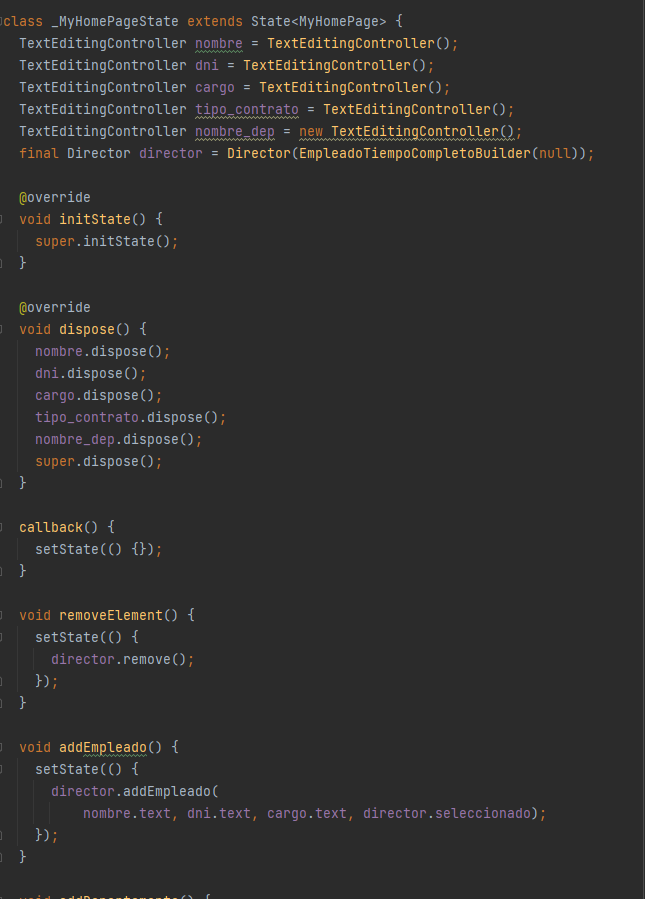
\includegraphics[width=5.90625in,height=8.03681in]{imagenes/main2.png}

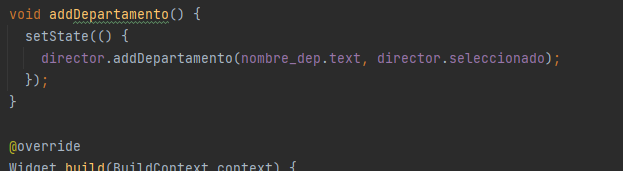
\includegraphics[]{imagenes/main3.png}

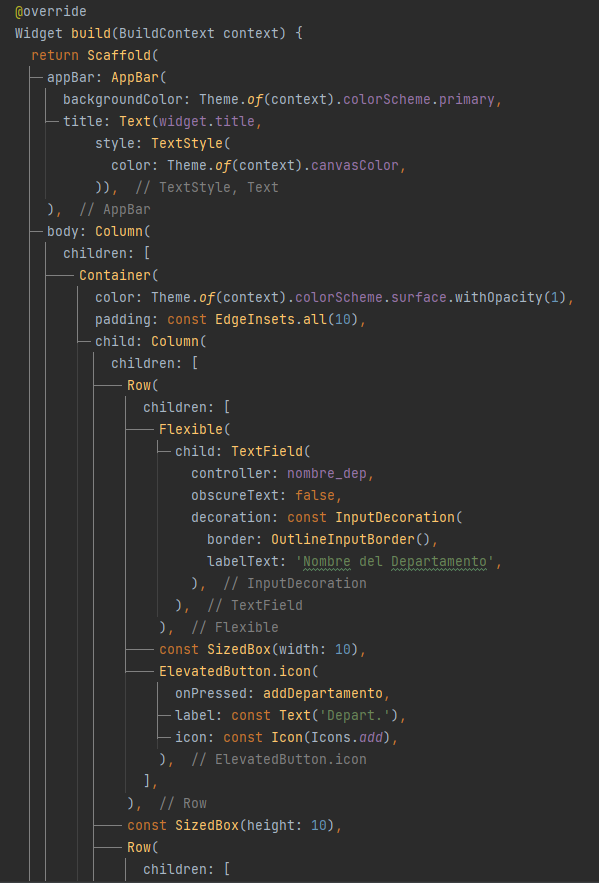
\includegraphics[width=5.90522in,height=8.70833in]{imagenes/main4.png}
\pagebreak
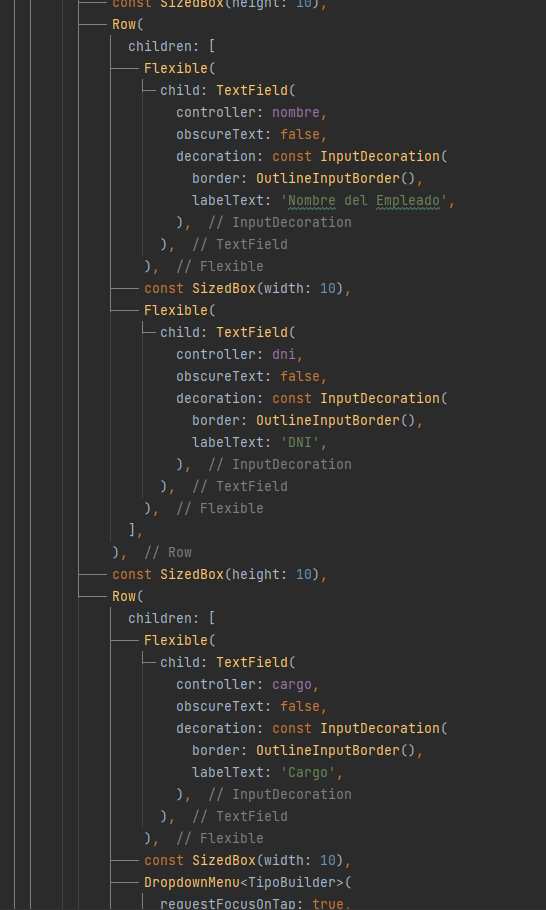
\includegraphics[width=5.6875in,height=9.47917in]{imagenes/main5.png}
\pagebreak
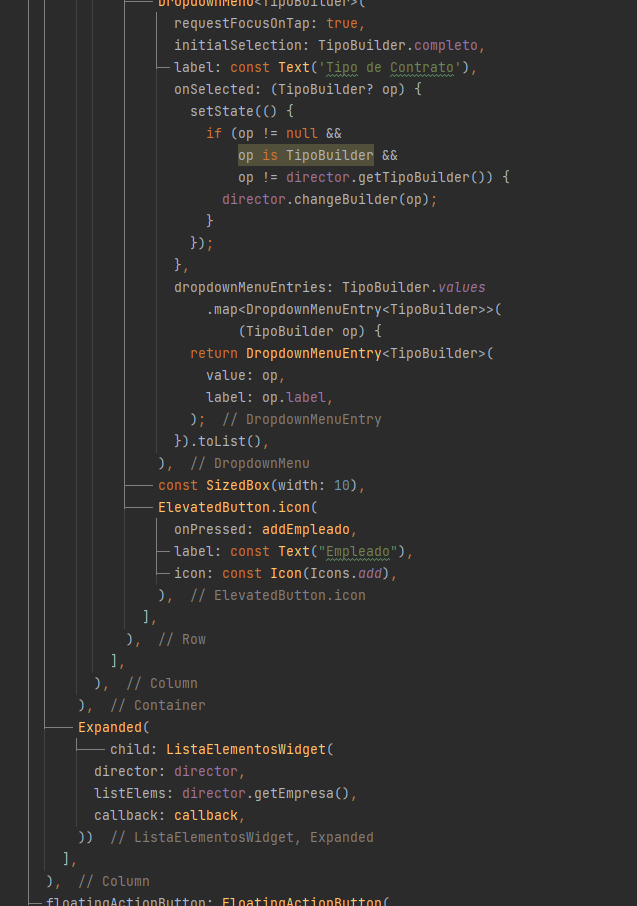
\includegraphics[width=5.90522in,height=8.40278in]{imagenes/main6.png}
\pagebreak
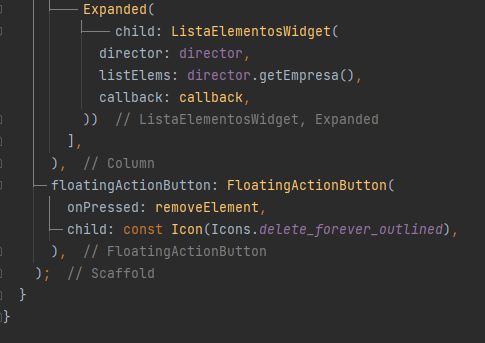
\includegraphics[]{imagenes/main7.png}

\section{\texorpdfstring{\hfill\break
}{ }}\label{section-1}

\section{Funcionamiento}\label{funcionamiento}

Ejemplo del funcionamiento.

Situación: Empresa de telemarketing, cuyos empleados trabajan desde sus
propias casas. Tienen un departamento para cada tipo de productos y una
sección de reclamaciones en cada una. Un empleado puede pertenecer a
varias divisiones.

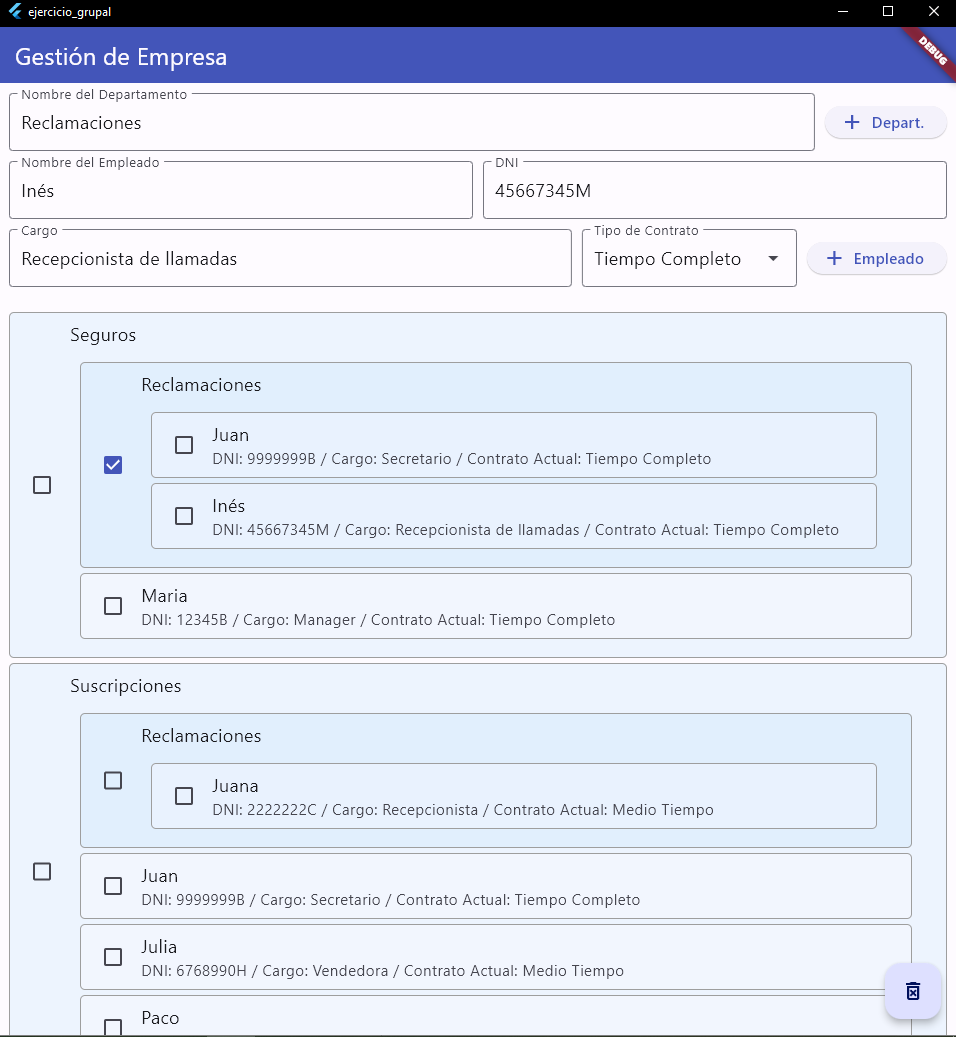
\includegraphics[width=5.90625in,height=6.19543in]{imagenes/Funcionamiento1.png}

Se puede hacer Scroll

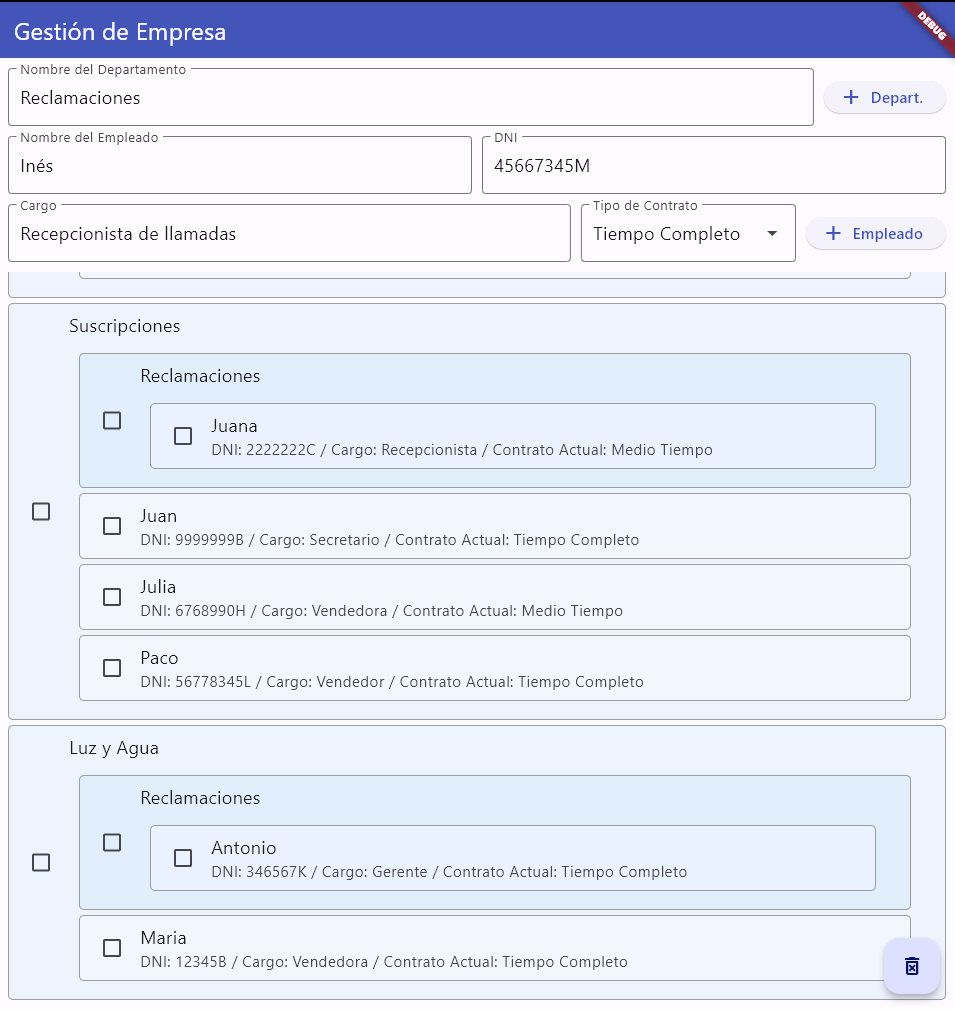
\includegraphics[width=5.90522in,height=6.23611in]{imagenes/Funcionamiento2.png}

Eliminamos algunos elementos (se puede eliminar un padre y sus hijos son
eliminados)

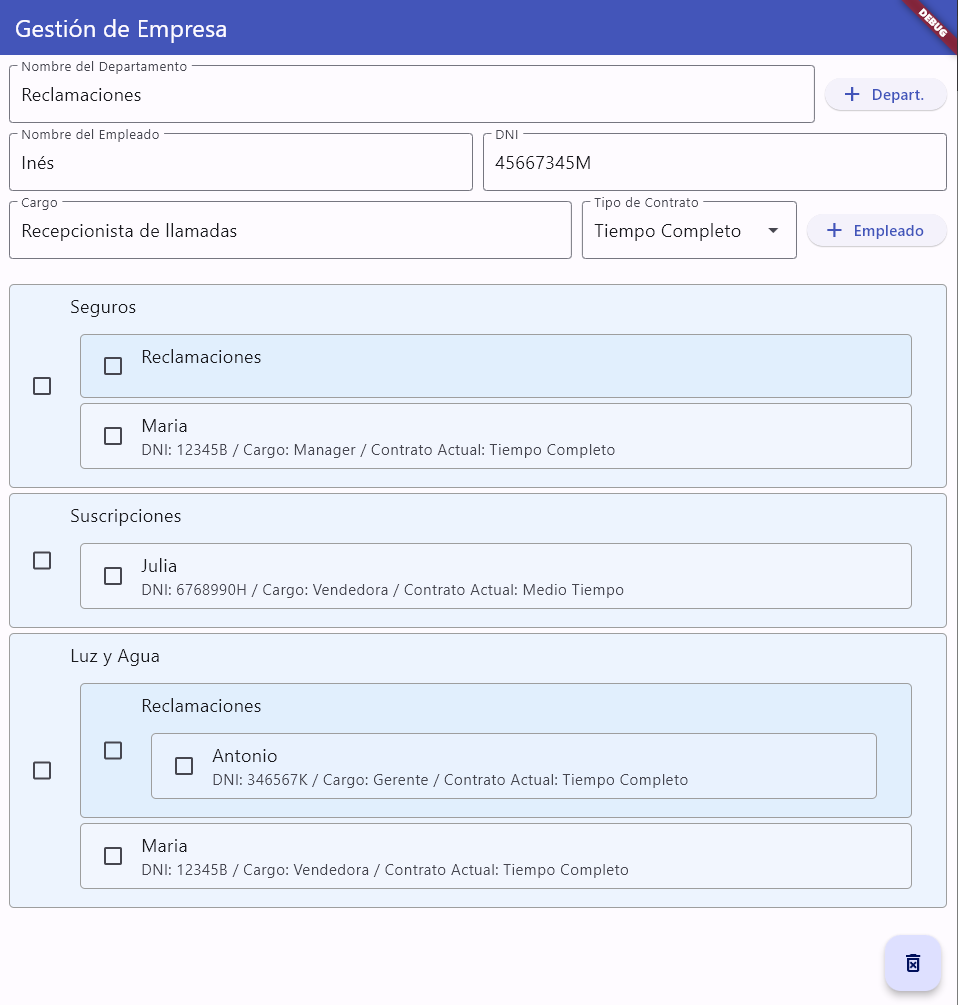
\includegraphics[width=5.90522in,height=6.19444in]{imagenes/Funcionamiento3.png}

Añadimos

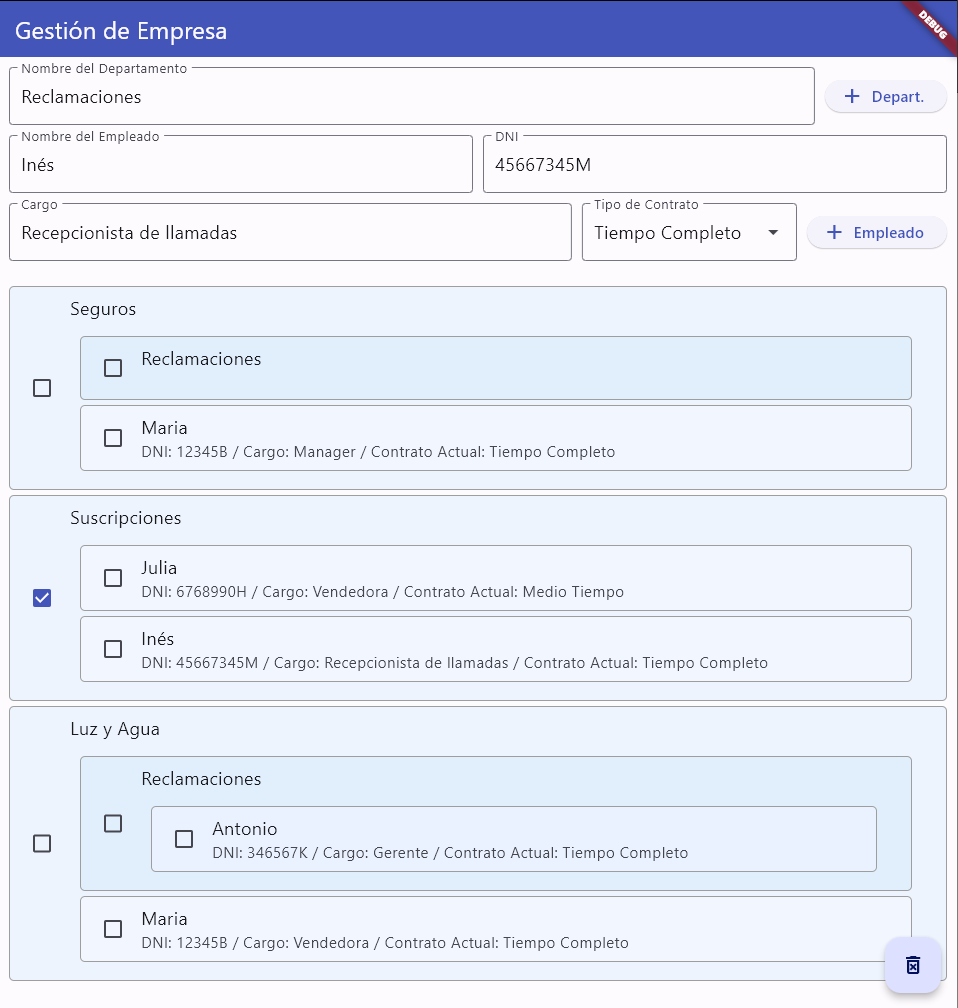
\includegraphics[width=5.90522in,height=6.20833in]{imagenes/Funcionamiento4.png}

\section{Conclusión}\label{conclusiuxf3n}

Para esta práctica se ha adaptado el código original y se ha rediseñado
para una aplicación que permite al usuario modificar los datos sin tocar
el código. El mayor cambio perfectivo que añade una nueva funcionalidad
es el hecho de que el director recuerde que ha sido seleccionado. Esto
es lo que permite los cambios desde la UI. Puesto que el modelo cuenta
con funciones para editar los valores, esa sería la mejora principal que
recibiría la aplicación en una supuesta expansión o quizá poder elegir
qué restricciones darle al director para la creación de elementos,
puesto que ahora mismo es bastante libre para poder adaptarse a muchas
estructuras de organización.

\end{document}

